\section{Desarrollo}

\subsection{Matriz normal}

Como una primera forma de resolución planeamos el parabrisas como un sistema de ecuaciones (más adelante veremos que el mismo presenta una organización de los elementos no nulos que se denomina $``banda"$, pero por ahora no tendremos en cuenta esto y por consiguiente no realizaremos ninguna optimización al respecto), este se vería representado como una matriz, donde cada columna representa a una posición especifica en el parabrisas pero que a su vez cada fila simboliza los coeficientes de las ecuaciones que se plantea para esa posición. Por lo tanto la diagonal de la matriz representa al coeficiente de esa posición en el parabrisas.
El parabrisas debe cumplir respetar 3 condiciones para el calculo de la temperatura.
La primera es que la temperatura del borde es de -100 grados, por lo que deberá respetarse la siguiente ecuación:

\begin{equation}
T(x,y) = -100^o\textrm{C}~~~~~\textrm{si } x = 0,m \textrm{ \'o } y = 0,n. 
\label{eq:borde}
\end{equation}
Donde m es ancho y n alto.\\
Y teniendo en cuenta que las sanguijuelas tienen una temperatura fija, las posiciones que las contengan deberán respetar la siguiente ecuación:
 \begin{equation}
T(x,y) = temp_{sanguijuela}
\label{eq:borde}
\end{equation}

Además, cada celda vacía es el promedio de las 4 contiguas, por lo que la ecuación a plantear es la siguiente:
\[
t_{ij} = (t_{i+1 j} + t_{i j+1} + t_{i-1 j} + t_{i j-1}) / 4
\]

\[
4 t_{ij} = t_{i+1 j} + t_{i j+1} + t_{i-1 j} + t_{i j-1}
\]

\[
 - 4 t_{ij} + t_{i+1 j} + t_{i j+1} + t_{i-1 j} + t_{i j-1}  = 0
\]

Nos queda que los coeficientes de la celda actual es -4 y de las contiguas un 1, igualando todo a cero.
Por lo tanto en cada fila de la matriz calculamos la posición que debería quedar sobre las celdas contiguas en nuestro sistema de ecuaciones.
Cada fila de nuestro sistema tendrá el siguiente aspecto

\[ \left( \begin{array}{ccccccccccc}
0 & ... & 0 & 1 & 0  & ... & 0 = -100 \end{array} 
\right)\] 


\[ \left( \begin{array}{ccccccccccc}
 0 &... & 0 & 1 & 0  & ... & 0 = temp_{sanguijuela} \end{array} 
\right)\] 



\[ \left( \begin{array}{cccccccccccccccccc}
0 & .. & 0 & 1 & 0 & ... & 0 & 1 & -4 & 1 & 0  & ... & 0 & 1 & 0 & .. & 0 = 0 \end{array} 
\right)\] 

 

Por lo tanto la solución a este sistema planteado se hará por medio del clásico método de resolución de Eliminación Gaussiana que consta de la eliminación progresiva de variables en el sistema de ecuaciones, hasta tener sólo una ecuación con una incógnita. Una vez resuelta esta, se procede por sustitución regresiva hasta obtener los valores de todas las variables.

\begin{verbatim}
Class Windshield{
    resolveByGaussianElimination(){
         gaussianElimination();
         backSubstitution();
    } 
    gaussianElimination(){
        for rows k already been reduced
            iMax = findPivot();
            Swap rows k and imax;
            Force 0’s in column A[k+1..n-1][k];
    }
    backSubstitution(){
        for row from last to first:
            calculateFromNextOneExceptForLast()
    }
}
\end{verbatim}

\subsection{Matriz Banda}

En la sección anterior presentamos una forma de resolver nuestro problema representando el parabrisas como un sistema de ecuaciones y aplicando Eliminación Gaussiana. En este sección propondremos una optimización a esto. Y para eso primero necesitamos ver con qué cosas estamos tratando.

Empecemos con un ejemplo, en este caso  tenemos un parabrisas de 6x6 granulado en 1 y una sanguijuela de radio 1 con temperatura de 500 en la primera posición.

El parabrisas se vería representado así (hay que tener en cuenta que en realidad hay que espejarlo horizontalmente ya que para nosotros el eje de coordenadas se encuentra arriba a la izquierda):

\begin{figure}[htb]
\begin{center}
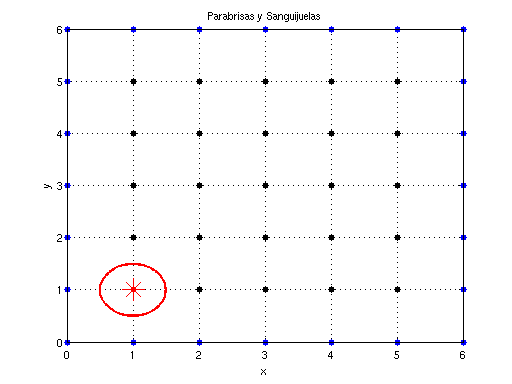
\includegraphics[scale=0.40]{imagenes/matrizbandaej_instancia.png} 
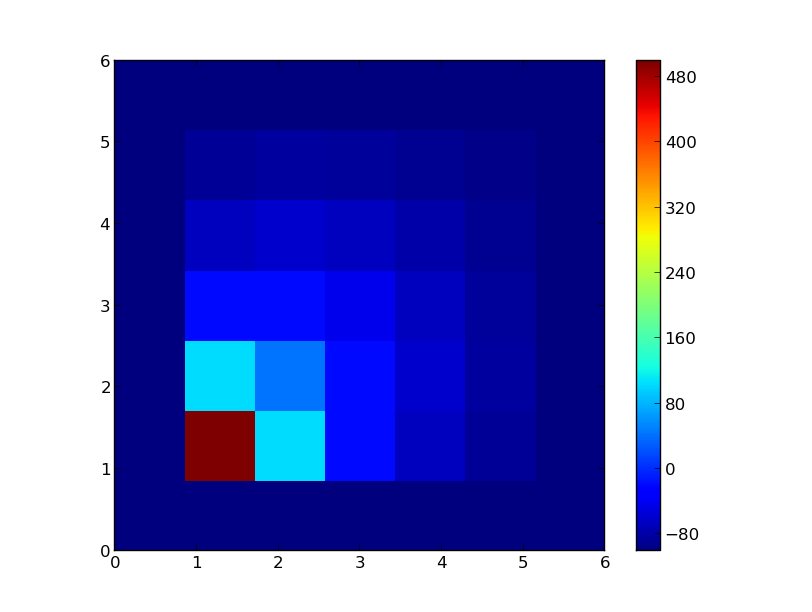
\includegraphics[scale=0.40]{imagenes/matrizbandaej_temp.png} 
\end{center}
\end{figure}

Con lo que el sistema quedaría de la siguiente forma: \\
(donde los espacios vacios representan blancos)
\begin{figure}
\begin{center}
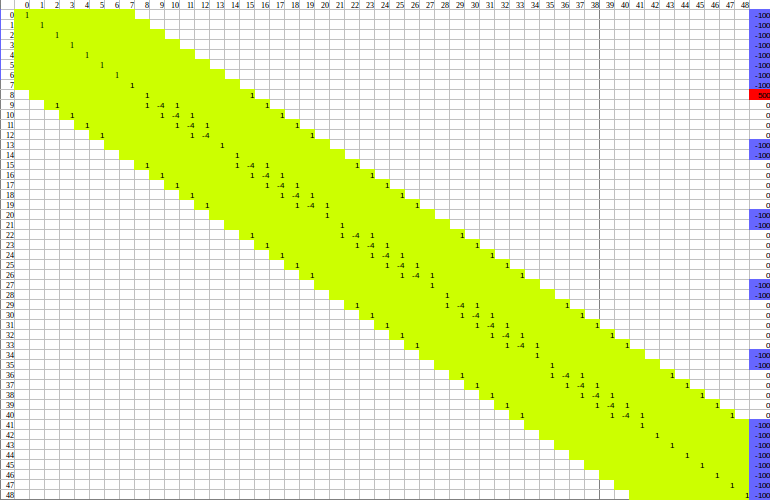
\includegraphics[scale=0.60]{imagenes/matrizej.png} 
\caption{Matriz de ecuaciones del ejemplo} 
\end{center}
\end{figure}


\newpage


Analizando la matriz del sistema de ecuaciones que se genera a partir de la representación del parabrisas observamos que presenta las características de la matriz $``banda"$ explicada anteriormente. 
Este es un hecho importante ya que las matrices banda tienen características especiales (como vimos anteriormente) por las cuales es posible la optimización temporal y espacial para resolver el sistema de ecuaciones con eliminación gausseana. Además también tiene la característica de ser semi definida positiva, lo que hace que no sea necesario swapear filas.
\subsubsection{Optimización}

El problema de representar la matriz original es que la mayoría de los valores son 0 y solo importan los elementos de la banda de la matriz, por lo tanto una forma de optimizar espacialmente es solo guardar la banda, con lo que se logra reducir considerablemente el espacio en esta representación, ya que suponiendo que se tiene un parabrisas de $n$ filas y $m$ columnas, el tamaño de la matriz original sería de $(n*m)^2$, mientras que con la optimización de matriz banda queda de tamaño $(n*m)*(2*m+1) \approx (n*m^2)$ .

El método para construir la representación optimizada de la matriz banda es simple, se guarda la banda en una matriz pero rotándola de forma que quede vertical.  Además se adiciona una columna más para representar la temperatura en esa posición.
Aunque uno podría pensar que ya que solo hay 5 elementos no nulos máximo en cada fila se podría optimizar guardando esos 5 coeficientes, pero debido a que luego se le aplicará el método de Back Substitution de la Eliminación Gausseana como método para resolver el sistema, esto hará que se generen valores no nulos dentro de la banda, por lo tanto el tamaño de esta matriz deberá ser lo suficiente como para poder trabajar sobre él y almacenar los valores parciales.
La matriz banda tendrá hasta un máximo de 5 valores no nulos por fila dependiendo el tipo de posición de la misma, ya que si en la posición hace referencia al borde frío, esta fila tendrá un 1 como valor central y un -100 en la columna de resultados, esto se deduce a partir de la expresión 
\begin{equation}
T(x,y) = -100^o\textrm{C}~~~~~\textrm{si } x = 0,m \textrm{ \'o } y = 0,n. 
\label{eq:borde}
\end{equation}
Donde m es ancho y n alto.\\
 El caso para el cual la posición contenga una sanguijuela será similar al de frío, ya que deberá respetar la ecuación
 \begin{equation}
T(x,y) = temp_{sanguijuela}
\label{eq:borde}
\end{equation}

Y por último, en base a las ecuaciones que deben respetar las posiciones vacías vistas anteriormente, en la posición central que representa a la posición actual quedará un -4 y en las de arriba-abajo-izquierda-derecha un 1 en cada una, siendo referenciadas en la matriz banda por las posiciones de la izquierda y derecha de la central, y las que están a distancia de la banda, por lo tanto, en las puntas de la fila de matriz, y al final de todo un 0 en la columna de resultado. Por lo tanto, cada fila que represente a una posición vacía tendrá una distribución inicial de la siguiente forma:


\[ \left( \begin{array}{ccccccccccc}
1 & 0 & ... & 0 & 1 & -4 & 1 & 0  & ... & 0 & 1\end{array} 
\right)\] 

El algoritmo consta de dos etapas, la construcción de la matriz que representara la banda y la resolución del problema utilizando la misma.

\paragraph{Construcción de la matriz banda}
\begin{verbatim}

por cada posición del parabrisas //O(N*M)
       pos = fila posición + columna posición * ancho;
		
              si en esa posición hay una SANGUIJUELA:
			
                    matrizBanda[pos][ancho] = 1;
                    resultados[pos]         = temp_sanguijuela;
		
              si esa posición es borde FRIO:
                    
                    matrizBanda[pos][ancho] = 1;
                    resultados[pos]         = -100;

              en caso de que esa posición sea VACIA:
                    
                    matrizBanda[pos][ancho]   = -4;
                    matrizBanda[pos][ancho-1] = 1;
                    matrizBanda[pos][0]       = 1;
                    matrizBanda[pos][ancho+1] = 1;
                    matrizBanda[pos][ancho*2] = 1;
                    resultados[pos]           = 0; 
		

\end{verbatim}

Continuando con el ejemplo que propusimos cuando empezamos esta sección, la matriz banda resultante sería la siguiente:

\begin{figure}
\begin{center}
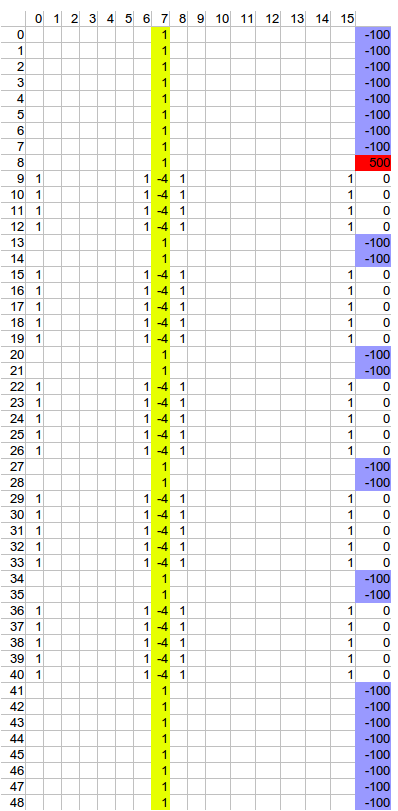
\includegraphics[scale=0.70]{imagenes/matrizbandaej.png} 
\caption{Matriz banda del ejemplo} 
\end{center}
\end{figure}

\newpage

Aquí se puede observar mejor como se distribuyen los coeficientes de la matriz original que pertenecen a la banda sobre esta nueva representación de ella, y como se $``verticaliza"$ la misma. Como sucedió anteriormente, los espacios en blanco representan los valores nulos.

Hasta este punto tenemos construida la representación de la matriz original en una forma que optimice el almacenamiento de la misma, ahora solo queda resolverla de una forma también optima.

\paragraph{Resolución del sistema} \mbox{}\\

Este algoritmo se basa básicamente en el algoritmo de eliminación gausseana para triangular y luego realizar un back sustitution para obtener el valor de los coeficientes.
Lo que es remarcable es el hecho de como trabaja en la matriz banda vertical como si fuese la banda en diagonal de la matriz original y la no necesidad de tener que intercambiar filas durante el proceso.
 
\begin{verbatim}

//PRIMERO LA HAGO TRIANGULAR SUPERIOR
PARA CADA FILA DE LA BANDA, DE ARRIBA A ABAJO:
		
   SI NO ES VACIO SE QUE ABAJO HAY TODO CERO, CONTINUO;
   SI ES VACIA DIAGONALIZO:
   {
         centro = bandMatrix[i][n];
         actual = bandMatrix[i+h][n-h];
         multiplicador = actual / centro;		
         fila[i+h] - fila[i];
         resultado[i+h] -= resultado[i] * multiplicador;
    }
   
 // EN ESTE PUNTO YA TENGO LA MATRIZ TRIANGULADA SUPERIORMENTE
 //AHORA SOLO FALTA REALIZAR
 // BACK SUBSTITUTION
 PARA CADA FILA i DE LA BANDA, DE ABAJO A ARRIBA
        fila = i / n;
        columna = i % n;
        for( int h = 1; h <= n; h++){ 
        // Recorro la banda en forma diagonal
        // Equivale a recorrer en forma vertical con la matriz normal
        // COMO ES BANDA ME FIJO SI EN LA DIAGONAL IZQ INF HAY DISTINTO DE 0 PARA PIVOTEAR
             centro = bandMatrix[i][n];
             actual = bandMatrix[i-h][n+h];           
             multiplicador = actual / centro;
		
             fila[i-h] -=  fila[i] * multiplicador; // Opero entre filas
             resultado[i-h] -= resultado[i]* multiplicador; 
                
             // y por último actualizo los valores del parabrisas con las temperaturas actuales             
             Parabrisas[fila][columna].temp = actual
       }
\end{verbatim}





\section{Eliminar sanguijuelas}

La resolución del problema de evitar el punto crítico en el centro del parabrisas consiste en la eliminación de sanguijuelas. Suponiendo la existencia de $n$ sanguijuelas, la cantidad de subconjuntos a probar son $2^n$. Es un número que crece rápidamente y si bien se puede resolver por fuerza bruta (ayudados por Backtracking y derivados), suponemos que encontrar el mínimo tiene un orden exponencial en la cantidad de sanguijuelas.

Finalmente, planteamos dos tipos de solución a modo de comparación. Estos serán detallados más adelante. Ambas son heurísticas por lo mencionado anteriormente.

\subsection{Punto Crítico}
En un parabrisas real el punto crítico se determina por el punto exacto del medio del parabrisas, en la posición (largo/2, ancho/2), pero en nuestra estructura de datos que representa al parabrisas esta puede no llegar a tener un punto exacto dependiendo de la discretización que tenga el mismo. Por lo tanto decidimos tomar la celda de la posición (filas/2,columnas/2), ya que en nuestra discretización sería una buena aproximación al centro. En caso de haber fila o columna impar tomamos la parte entera de la división.

\subsection{Solución Greedy}
Esta solución consiste en ir seleccionando las sanguijuelas más cercanas al punto medio hasta que el punto central esté por debajo de 235 Cº. Al no ser una solución exacta es posible que eliminar la más cercana al centro no pertenezca a la mejor solución, pero es intuitivo suponer que la sanguijuela que más cause calor al punto medio esté cerca del mismo. \\
Lo primero que se realiza es ordenar las sanguijuelas según su distancia al centro. Para esto utilizamos la función $sort()$ de C++ que utiliza como comparador el valor pre-calculado de distancia al centro. El orden de esta parte es $O(n.log(n))$ en donde n es la cantidad de sanguijuelas.\\
Al ser una solución golosa (greedy), elige la siguiente sanguijuela siempre y cuando no se haya enfriado el punto medio y haya salido del estado crítico. La elección está dada por la sanguijuela más cerca todavía no elegida en una previa iteración.\\
Suponiendo que la complejidad de rehacer el cálculo es $RA$, la complejidad final es:  $O(n.log(n) + n*RA)$. Notar que esa última $n$ es en el peor caso que tengamos que eliminar todas las sanguijuelas, pero debería ser un $k < n$.



\begin{algorithm}
\caption{Solución Greedy}\label{euclid}
\begin{algorithmic}[1]
\State $\textit{ordenoLasSanguijuelasPorCercaníaAlPuntoCrítico() }$
\State $\textit{sanguijuelasAMatar} \gets []$
\Do
    \State sanguijuelasAMatar.agregar(obtenerSanguijuelaMasCercana())
  \doWhile{$ laTemperaturaEsAlta()$} % <--- use \doWhile for the "while" at the end
\State $\textit{devuelvo sanguijuelasAMatar}$
\end{algorithmic}
\end{algorithm}

\begin{algorithm}
\caption{laTemperaturaEsAlta()}\label{euclid}
\begin{algorithmic}[1]
\State $\textit{recalculoConMatrizBanda();}$
\State $\textit{devuelvo (parabrisas.tempPuntoCritico() $>$ 235)}$
\end{algorithmic}
\end{algorithm}


\subsubsection{Espiral vs centrico}
	Durante el desarrollo del algoritmo Greedy, nuestro primer acercamiento fue recorrer la matriz de forma espiral. El primer problema que encontramos fue que teníamos un cálculo muy grande para determinar dado un punto del parabrisas, qué sanguijuela era y que recorríamos partes de la matriz que no importaban (en especial los bordes). A su vez, tendíamos a alejarnos del objetivo principal que era preocuparnos por el centro. Es por eso que decidimos ordenar las sanguijuelas según su distancia al centro. Para ahorrar tiempo computacional, este dato está calculado en el momento de la creación de la sanguijuela para su posterior ordenamiento.

\subsection{Solución Random}\label{sec:solucionRandom}
En esta solución seleccionamos de nuestro array de posiciones de sanguijuelas (que es el array recibido por parámetro, con las posiciones sin discretizar) una al azar y la eliminamos. Luego ejecutamos de nuevo el cálculo de las temperaturas y chequeamos si el punto crítico esta por debajo del 235 Cº.Si no lo está, elegimos otra al azar y repetimos el proceso hasta que lo esté. 

\begin{algorithm}
\caption{RandomSolution}\label{euclid}
\begin{algorithmic}[1]
\Do
    \State matarSanguijuelaRandom()
  \doWhile{$laTemperaturaEsAlta()$} % <--- use \doWhile for the "while" at the end
\State $\textit{return sanguijuelasAEliminar}$
\end{algorithmic}
\end{algorithm}

\begin{algorithm}
\caption{matarSanguijuelaRandom()}\label{euclid}
\begin{algorithmic}[1]
\State $\textit{sanguijuelasAEliminar.agregar(removerSanguijuelaRandom(listaSanguijuelas));}$ \Comment{All Leaches is loaded with matrix}
\State $\textit{recalculoConMatrizBanda();}$
\end{algorithmic}
\end{algorithm}

